% LaTeX document class and template packages
\documentclass[10pt,twocolumn,twoside]{article}
\usepackage[margin=0.75in]{geometry}
\usepackage{url}
\usepackage{color}
\usepackage{amsmath}
\usepackage{algorithm}
\usepackage{algorithmicx}
\usepackage{graphicx}
\usepackage[numbers,sort&compress,comma]{natbib}
\usepackage[colorlinks=true,linkcolor=blue,citecolor=blue,urlcolor=blue]{hyperref}
\usepackage{nameref} % nameref must be after hyperref

% LaTeX document preamble and commands
\newcommand{\etal}{\textit{et al.}}
\pagestyle{myheadings}
\date{} % filename BHAVI2016JLCT.tex
\author{Jason~J.~Liu, Adam~Craig, and Carl~Taswell}
\title{Using MongoDB and Mongoose with a MEAN Stack Implementation of the NEXUS-PORTAL-DOORS System\\ } 
\markboth{J.~J.~Liu \etal}{BHA-2016-06 ver \today}

% LaTeX document
\begin{document}
\maketitle
\thispagestyle{empty}

\section*{Introduction}
\label{secIntroduction}
	For researchers, primary research is only the first stepping stone to proving or disproving a theory. One successful experiment proves little to nothing in the grand scheme of the scientific community. However, the weakness of a single experiment is covered by the power of the meta-analysis, usually completed by a third party. Meta-analysis requires researchers to analyze results from muliple primary articles and assess whether or not the result is accurate, show if the hypothesis presented are proven or disproven, and provide a degree of error. However, despite the necessity of meta-analyses, it continues to be time consuming and ineffective at connecting with all points of data. The miniscule amount of secondary articles pale in comparison to the literal thousands of primary articles which are published each day. In order to take advantage of all the new information which is provided and to create more effective secondary analyses, a semantic web solution provides the necessary tools in order to take full statistical advantage that meta-analysis offers. 
 \newline
	In order to support PORTAL registries and DOORS directories, a database is necessary in order to support and store the data. In order to take full advantage of a tried and true framework, MEAN stack serves as the ideal system by thoroughly integrating client-side, server-side, and database processes. 

\section*{Methods}
\label{secMethods}
	For this new NEXUS-PORTAL-DOORS (NPD) system implementation, both backend and front end will rely heavily on node.js, an open-source runtime environment which enables scalable web applications and servers. Used with Express and other packages, node.js enables the user to organize a web application into a MVC (model-view-controller) architecture. In accordance with the "M" from MEAN stack, MongoDB serves as the database for the NPD. However, MongoDB acts only as a database, offering a bare minimum in regards to complex and automated queries. Mongoose enables connection to a MongoDB database from javascript, allowing model abstraction, large scale queries, data validation, and more. It also creates an SQL style database through schemas, creating a structured system in a NoSQL database. 
\begin{figure*}[ht]
{\centering
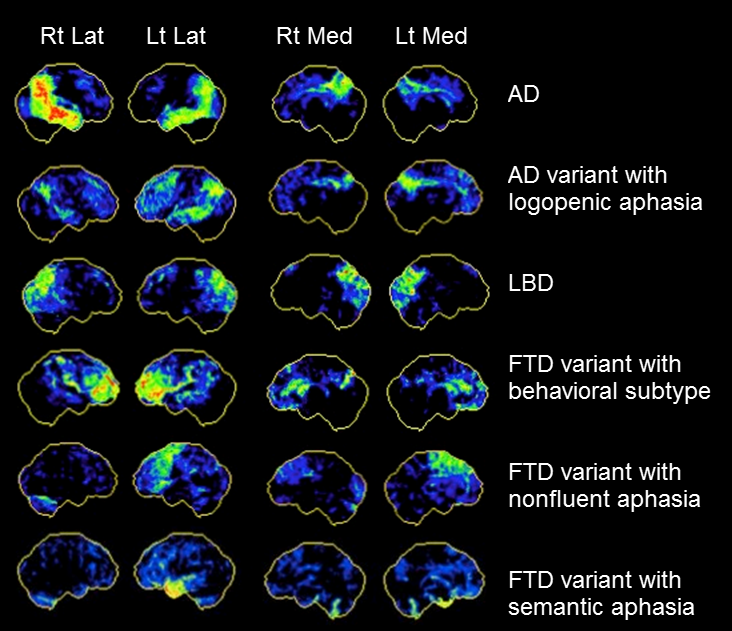
\includegraphics[width=6.5in]{FDGPETFOD_patterns_ctrev3.png}
\caption{FDG-PET scan patterns displayed in NeuroStat 3D-SSP for focal onset dementias.}
\label{figADPatterns} }
\end{figure*}


\section*{Results}
\label{secResults}
Table~\ref{tabPatDemo} 
\begin{table*}[ht]\begin{center}
\caption{Patient Demographics for Selected Subgroups in Study Cohort}
\label{tabPatDemo}
\begin{tabular}{l l r | c c | c c  }
\multicolumn{3}{c|}{Subgroup selected by diagnostic marker} 
	& \multicolumn{2}{c|}{Sex} & \multicolumn{2}{c}{Age at PET Scan} \\ \hline
Subgroup Id      & Description                    & N  & Male & Female & Median & Min -- Max \\ \hline
1                & C11-PiB Imaging AD             & 51 & 27   & 24    & 65 & 53 -- 81 \\
2                & F18-FDG Imaging AD             & 49 & 22   & 27    & 65 & 53 -- 81 \\
3                & Clinical AD                    & 24 & 13   & 11    & 69 & 56 -- 81 \\
4                & Clinical PPA-L (AD variant)    & 19 &  7   & 12    & 67 & 53 -- 78 \\
5                & Clinical PPA-G                 & 16 & 12   &  4    & 71 & 48 -- 80 \\
6                & Clinical PPA-S                 & 13 &  8   &  5    & 64 & 54 -- 77 \\
7                & Clinical CBS                   & 14 &  6   &  8    & 64 & 57 -- 73 \\
8 (pooled 3--4)  & Clinical AD \& PPA-L           & 43 & 20   & 23    & 69 & 53 -- 81 \\
9 (pooled 5--7)  & Clinical PPA-G, PPA-S \& CBS   & 43 & 26   & 17    & 66 & 48 -- 80 \\
10               & Entire cohort                  & 94 & 52   & 42    & 68 & 37 -- 81 \\
\end{tabular}\end{center}\end{table*}
summarizes the sample sizes and demographics for each of 
the selected subgroups of patients analyzed in the study cohort.


\section*{Discussion}
\label{secDiscussion}
discussion text here


\section*{Conclusion}
\label{secConclusion}
conclusion text here


\section*{Acknowledgments}
Do not acknowledge co-authors; only acknowledge persons who have contributed
to or otherwise supported the study in some way but did not get recognized as a co-author.
Acknowledgments are also used to identify any outside funding sources other than
the affiliated institution identified for authors.


\section{References}
\begin{enumerate}
\item Barrasa Rodriguez, J., Corcho, �. and G�mez-P�rez, A.
R2O, an extensible and semantically based database-to-ontology mapping language
Springer-Verlag, 2004
\item Berners-Lee, T., Hendler, J., Lassila, O. and others
The semantic web
Scientific american, New York, NY, USA:, 2001, Vol. 284(5), pp. 28-37
\item Dickey, J.
Write modern web apps with the MEAN stack: Mongo, Express, AngularJS, and Node. js
Pearson Education, 2014
\item MySQL, A.
MySQL
2001
\item Pan, Z. and Heflin, J.
Dldb: Extending relational databases to support semantic web queries
DTIC Document, DTIC Document, 2004
\item Spanos, D.-E., Stavrou, P. and Mitrou, N.
Bringing relational databases into the semantic web: A survey
Semantic Web, IOS Press, 2012, Vol. 3(2), pp. 169-209
\item Stojanovic, L., Stojanovic, N. and Volz, R.
Migrating data-intensive web sites into the semantic web
Proceedings of the 2002 ACM symposium on Applied computing
2002, pp. 1100-1107
\item Suehring, S.
MySQL bible
John Wiley and Sons, Inc., 2002
\item Taswell, C.
DOORS to the semantic web and grid with a PORTAL for biomedical computing
IEEE Transactions on Information Technology in Biomedicine, IEEE, 2008, Vol. 12(2), pp. 191-204
\item Taswell, C.
Portals and doors for the semantic web and grid
Google Patents, 2010
\item Taswell, C.
A distributed infrastructure for metadata about metadata: The HDMM architectural style and PORTAL-DOORS system
Future Internet, Molecular Diversity Preservation International, 2010, Vol. 2(2), pp. 156-189
\end{enumerate}


% References: note that the \nocite{*} command will automatically generate 
%  a reference list for all references contained in all *.bib files separated by
%  commas in the \bibliography{} command.
\nocite{*}
\bibliographystyle{plainnat}
\bibliography{BrainWarping}
\end{document}